\section{Lecture 8. Graph Pattern Mining}

\subsection{Frequent (Sub)Graph Patterns}
Given a labeled graph dataset $D = \{G_1, G_2, ..., G_n\}$, the supporting graph set of a subgraph g is $D_g = \{G_i \mid g \subseteq G_i, G_i \in D \}$:
\begin{equation*}
support(g) = \abs{D_g} / \abs{D}
\end{equation*}

A (sub)graph g is frequent if $support(g) \geqslant min\_sup$.

\begin{figure}[H]
    \centering
    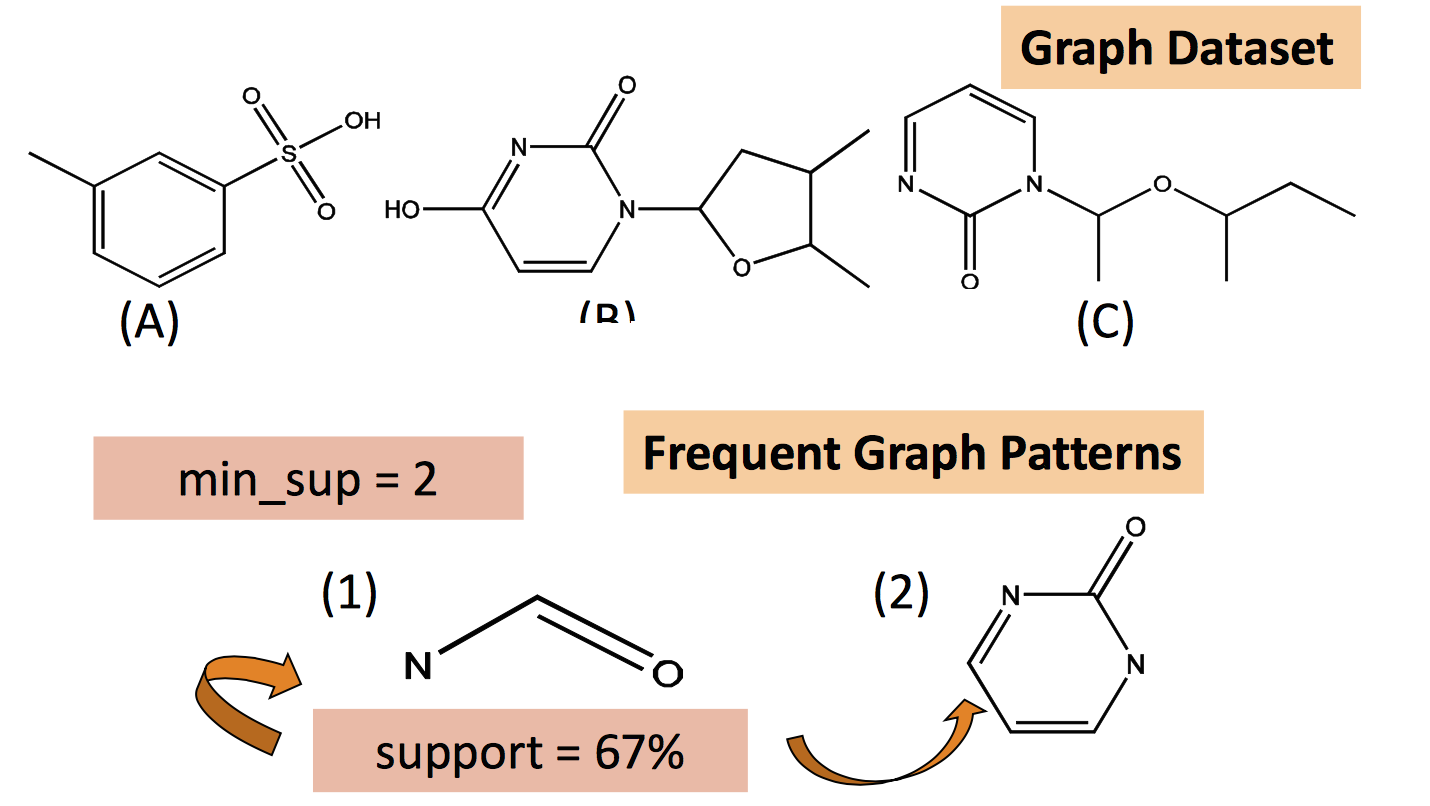
\includegraphics[width=\linewidth]{chemical_structures.png}
    \caption{Example: Chemical structures}
\end{figure}

%--
\subsection{Apriori-Based Approach}

\textbf{The Apriori property} (anti-monotonicity): a size-k subgraph is frequent if and only if all of its subgraphs are frequent.\\

Candidate generation: a candidate size-(k+1) edge/vertex subgraph is generated if its corresponding two k-edge/vertex subgraphs are frequent:
\begin{itemize}
\item AGM - Generating new graphs with one more vertex
\item FSG - Generating new graphs with one more edge (more efficient)
\end{itemize}

Iterative mining process: Candidate-generation $\to$ candidate pruning $\to$ support counting $\to$ candidate elimination.

%--
\subsection{gSPAN: Graph Pattern Growth}
Depth-first growth of subgraphs from k-edge to (k+1)-edge, then (k+2)-edge subgraphs generates many duplicate subgraphs.\\

\textbf{Right-most path extension} in subgraph pattern growth reduces generation of duplicate subgraphs: \textit{take the path from root to the right-most leaf (choose the vertex with the smallest index at each step)}. The Enumeration of graphs using right-most path extension is complete.\\

DFS Code: flatten a graph into a sequence using depth-first search

\begin{figure}[H]
    \centering
    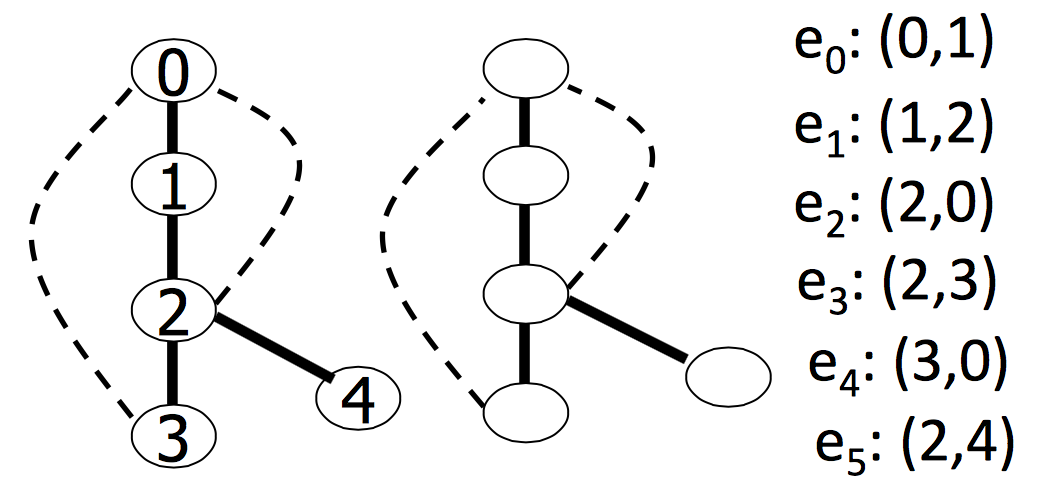
\includegraphics[width=0.8\linewidth]{gspan.png}
    \caption{gSPAN}
\end{figure}

%--
\subsection{Mining Closed Graph Patterns}

A frequent graph G is closed if there exists no supergraph of G that carries the same support as G.\\

\textbf{CloseGraph} algorithm: mining closed graph patterns by extending gSpan. Suppose G and $G_1$ are frequent, and G is a subgraph of $G_1$. If in any part of the graph in the dataset where G occurs, $G_1$ also occurs, then we need not grow G (except some special, subtle cases), since \textit{none of G’s children will be closed except those of $G_1$}.

%--
\subsection{gIndex: A Graph Indexing Method}

\begin{figure}[H]
    \centering
    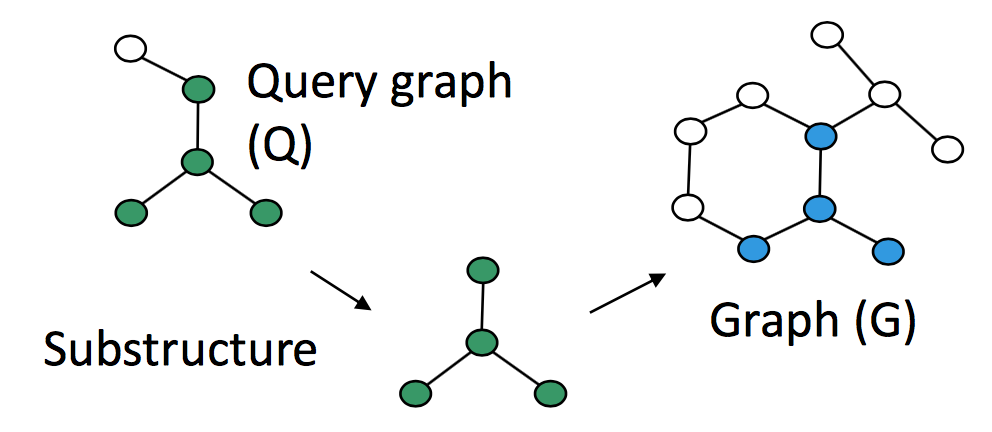
\includegraphics[width=0.8\linewidth]{gindex.png}
    \caption{Graph query}
\end{figure}

\begin{itemize}
\item use frequent substructures for indexing
\item discriminative substructures: reduce index size by removing similar (not discriminative) substructures from the index
\end{itemize}

\begin{definition}
Fragment x is \textbf{discriminative} with respect to feature set F if $D_x \ll \bigcap_{f \in F \wedge f \subseteq x}D_f$, where $D_x$ is the set of graphs containing x.
\end{definition}

Selection: Given a set of indexing features $f_1, f_2, .. f_n$, and a new structure x (x should be either redundant or discriminative), the extra indexing power is measured by occurrence probability 
\begin{equation*}
Pr(x \mid f_1,f_2,...f_n) = \frac{\abs{\bigcap_{f \in F \wedge f \subseteq x}D_f}}{\abs{D_x}}
\end{equation*}
When $Pr(x \mid f_1,f_2,...f_n) \ll 1$, x is a discriminative structure and should be included in the index.

%--
\subsection{SpiderMine: Mining Top-K Large Structural Patterns in a Massive Network}
\textbf{SpiderMine}: mine top-K largest frequent substructure patterns whose diameter is bounded by $_{Dmax}$ with a probability at least $1− \varepsilon$. General idea: large patterns are composed of a number of small components (<<spiders>>) which will eventually connect together after some rounds of pattern growth.\\

An r-spider is a frequent graph pattern P such that there exists a vertex u of P, and all other vertices of P are within distance r from u.\\

The SpiderMine Algorithm
\begin{itemize}
\item Mine the set S of all the r-spiders
\item Randomly draw M r-spiders
\item Grow these M r-spiders for $t = D_{max}/2$ iterations, and merge two patterns whenever possible
\item Discard unmerged patterns
\item Continue to grow the remaining ones to maximum size
\item Return the top-K largest ones in the result
\end{itemize}

SpiderMine general ideas:
\begin{itemize}
\item Small patterns are much less likely to be hit in the random draw
\item Even if a small pattern is hit, it is even less likely to be hit multiple times 
\item The larger the pattern, the greater the chance it is hit and saved
\end{itemize}


%--
\subsection{Recommended Readings}
\begin{itemize}
\item C. Borgelt and M. R. Berthold, <<Mining molecular fragments: Finding relevant substructures of molecules>>, ICDM'02
\item J. Huan, W. Wang, and J. Prins. <<Efficient mining of frequent subgraph in the presence of isomorphism>>, ICDM'03
\item A. Inokuchi, T. Washio, and H. Motoda. <<An apriori-based algorithm for mining frequent substructures from graph data>>, PKDD'00
\item M. Kuramochi and G. Karypis. <<Frequent subgraph discovery>>, ICDM'01
\item S. Nijssen and J. Kok. A quickstart in frequent structure mining can make a difference. KDD'04
\item N. Vanetik, E. Gudes, and S. E. Shimony. <<Computing frequent graph patterns from semistructured data>>, ICDM'02
\item X. Yan and J. Han, <<gSpan: Graph-Based Substructure Pattern Mining>>, ICDM'02
\item X. Yan and J. Han, <<CloseGraph: Mining Closed Frequent Graph Patterns>>, KDD'03
\item X. Yan, P. S. Yu, and J. Han, <<Graph Indexing: A Frequent Structure-based Approach>>, SIGMOD'04
\item F. Zhu, Q. Qu, D. Lo, X. Yan, J. Han, and P. S. Yu, <<Mining Top-K Large Structural Patterns in a Massive Network>>, VLDB'11
\end{itemize}